\documentclass[11pt,compress,t,notes=noshow, aspectratio=169, xcolor=table]{beamer}

\usepackage[nospeakermargin]{../../style/lmu-lecture-2}
% Defines macros and environments
% This file is included in slides and exercises

% Rarely used fontstyle for R packages, used only in 
% - forests/slides-forests-benchmark.tex
% - exercises/single-exercises/methods_l_1.Rnw
% - slides/cart/attic/slides_extra_trees.Rnw
\newcommand{\pkg}[1]{{\fontseries{b}\selectfont #1}}

% Spacing helpers, used often (mostly in exercises for \dlz)
\newcommand{\lz}{\vspace{0.5cm}} % vertical space (used often in slides)
\newcommand{\dlz}{\vspace{1cm}}  % double vertical space (used often in exercises, never in slides)
\newcommand{\oneliner}[1] % Oneliner for important statements, used e.g. in iml, algods
{\begin{block}{}\begin{center}\begin{Large}#1\end{Large}\end{center}\end{block}}

% Don't know if this is used or needed, remove?
% textcolor that works in mathmode
% https://tex.stackexchange.com/a/261480
% Used e.g. in forests/slides-forests-bagging.tex
% [...] \textcolor{blue}{\tfrac{1}{M}\sum^M_{m} [...]
% \makeatletter
% \renewcommand*{\@textcolor}[3]{%
%   \protect\leavevmode
%   \begingroup
%     \color#1{#2}#3%
%   \endgroup
% }
% \makeatother

\usepackage{pax}
\setbeamertemplate{frametitle}{\expandafter\uppercase\expandafter\insertframetitle}
%\useoutertheme{metropolis}
% remove section slides
\AtBeginSection[]
{
	\begin{frame}<beamer>
		\frametitle{Advanced Machine Learning}
		\tableofcontents[currentsection]
	\end{frame}
}
% includepdf slides, pagecommad will set counter for framenumber
\usepackage{pdfpages}
\includepdfset{trim=0mm 0mm 0mm 0mm, pagecommand={\global\setcounter{framenumber}{\value{page}}}}
% trim=0mm 6mm 0mm 0mm, offset=0 15,
% add footer:
\usepackage{framed, color}
\usepackage{xcolor}
%\iffalse
\setbeamertemplate{footline}[text line]{%
	\noindent\hspace*{\dimexpr-\oddsidemargin-1in\relax}%
	\colorbox{white}{
		\makebox[\dimexpr\paperwidth-2\fboxsep\relax]{
			\color{black}
			\begin{minipage}[c][2ex][c]{0.5\linewidth}
				\secname
			\end{minipage}
			\hfill\begin{minipage}[c][2ex][c]{0.5\linewidth}
				\flushright
				\insertframenumber{}~/~\inserttotalframenumber~~
			\end{minipage}
	}}%
	\hspace*{-\paperwidth}
}
%\fi
\title{Applied Machine Learning}
% \author{LMU}
%\institute{\href{https://compstat-lmu.github.io/lecture_iml/}{compstat-lmu.github.io/lecture\_iml}}
\date{}

\begin{document}

\newcommand{\titlefigure}{figure/empty}
\newcommand{\learninggoals}{
\item Imputation}

\lecturechapter{Imputation}
\lecture{Applied Machine Learning}

\section{Imputation}
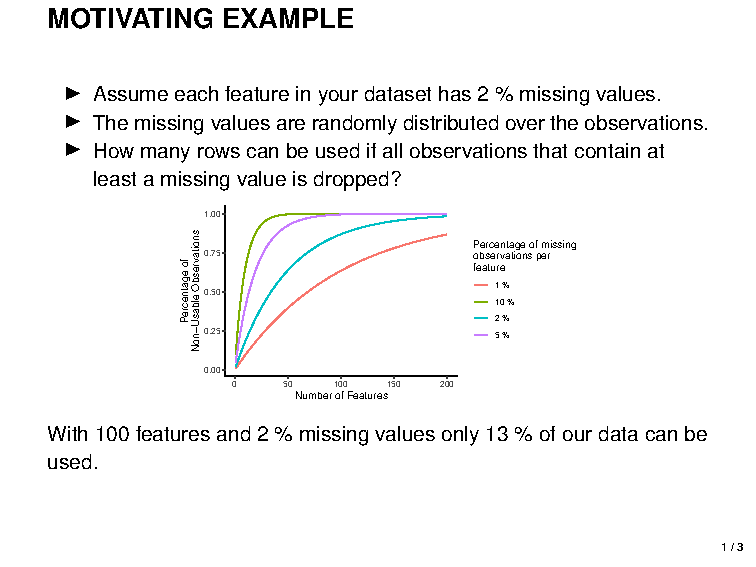
\includepdf[pages={1-2}]{pdf_chapters/slides_01_imputation_intro.pdf}
\begin{frame}{Why is data missing? \href{https://arxiv.org/pdf/2407.19804}{\beamergotobutton{REF}}}
    \vfill
    \begin{itemize}
        \item faulty measurements
        \item unanswered questionnaire items
        \item unreported data
    \end{itemize}
    \vfill
\end{frame}
\begin{frame}{Missingness mechanisms}
    \vfill
    \begin{itemize}
        \item MCAR (Missing Completely At Random)
        \begin{itemize}
            \item Data is missing independently of missing or observed values
        \end{itemize}
        \item MAR (Missing At Random)
        \begin{itemize}
            \item Missingness depends only on observed values
        \end{itemize}
        \item MNAR (Missing Not At Random)
        \begin{itemize}
            \item Missingness depends on observed and missing values
        \end{itemize}
    \end{itemize}    
    \vfill
    \pause
    Which one is most realistic to assume in the real world?
    \vfill
\end{frame}
\begin{frame}{Missingness mechanisms - Examples}
    \vfill
    \begin{itemize}
        \item MCAR (Missing Completely At Random)
        \begin{itemize}
            \item Participants skip a page of a questionaire because they flip two pages at once
        \end{itemize}
        \item MAR (Missing At Random)
        \begin{itemize}
            \item Certain medical examinations are conducted more often for certain patient groups (age groups, different gender)
            \item Certain demographic groups are less likely to fill in surveys about depression (but demographic groups is often fully observable, e.g., gender)
        \end{itemize}
        \item MNAR (Missing Not At Random)
        \begin{itemize}
            \item Missingness depends on observed and missing values
        \end{itemize}
    \end{itemize}    
    \vfill
\end{frame}
\includepdf[pages={3}]{pdf_chapters/slides_01_imputation_intro.pdf}
\begin{frame}{Reasons to impute missing values}
    \vfill
    \begin{itemize}
        \item Prediction
        \begin{itemize}
            \item Goal: allow for maximal predictive performance
        \end{itemize}
        \item Inference
        \begin{itemize}
            \item Goal: estimate parameters such as mean and variance of the variable distribution
            \item Not part of this lecture
        \end{itemize}
    \end{itemize}
    \vfill
    $\rightarrow$ 
    \begin{itemize}
        \item Imputation depends on the goal
        \item Imputation needs to be benchmarked wrt the downstream task
    \end{itemize}
    \vfill
\end{frame}

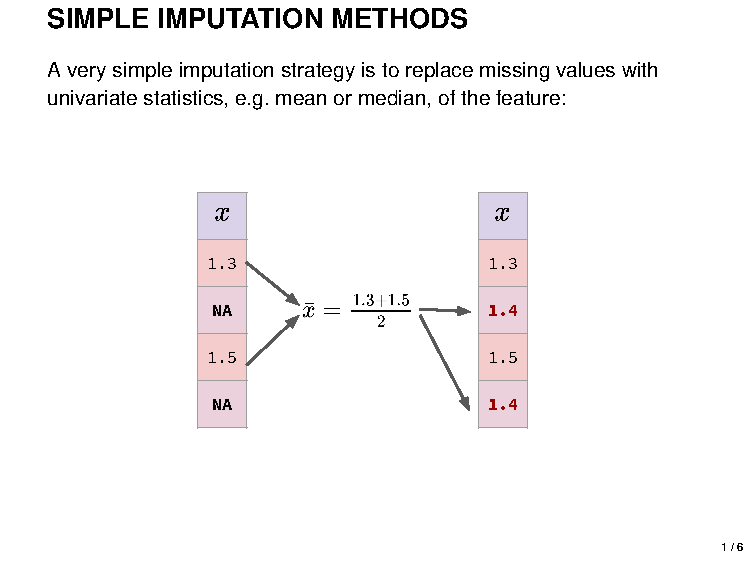
\includepdf[pages={1-2}]{pdf_chapters/slides_02_imputation_simple.pdf}
\begin{frame}{Imputation Notes}
\begin{itemize}
    \item  To ensure that the information regarding which values were imputed is not lost, we can add a binary indicator variable.
        \begin{itemize}
            \item Provides additional information in MNAR
        \end{itemize}
    \item Domain knowledge is highly important: Missing Credit can mean that the individual has 0 debt.
    \item Encoding numeric values with out-of-range values has been shown to work well in practice for complex ML models.
        \begin{itemize}
            \item This is especially useful for tree-based methods, as it allows separating observations with missing values in a feature.
            \item But using out-of-range imputation when estimating global effects (e.g. in linear models) can skew the results
        \end{itemize}
\end{itemize}    
\end{frame}

\includepdf[pages={4-6}]{pdf_chapters/slides_02_imputation_simple.pdf}
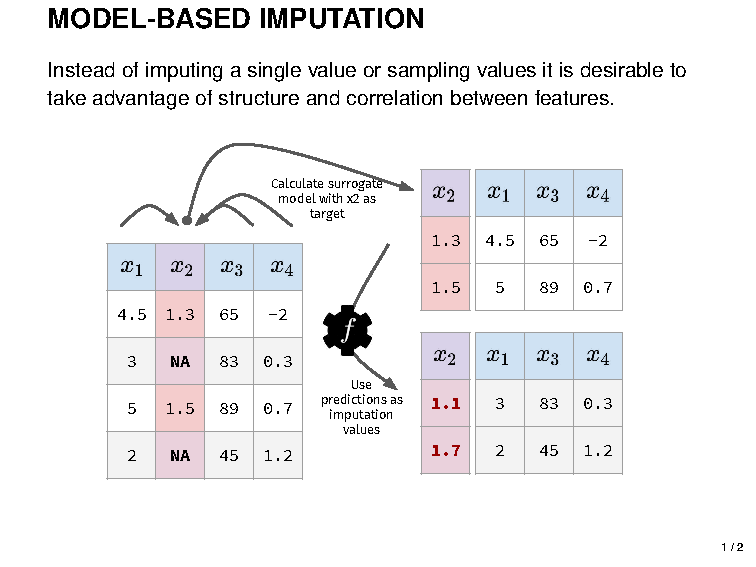
\includepdf[pages={1-last}]{pdf_chapters/slides_03_imputation_models.pdf}

\begin{frame}{A tale of failed imputation}
\vfill
\begin{figure}
    \centering
    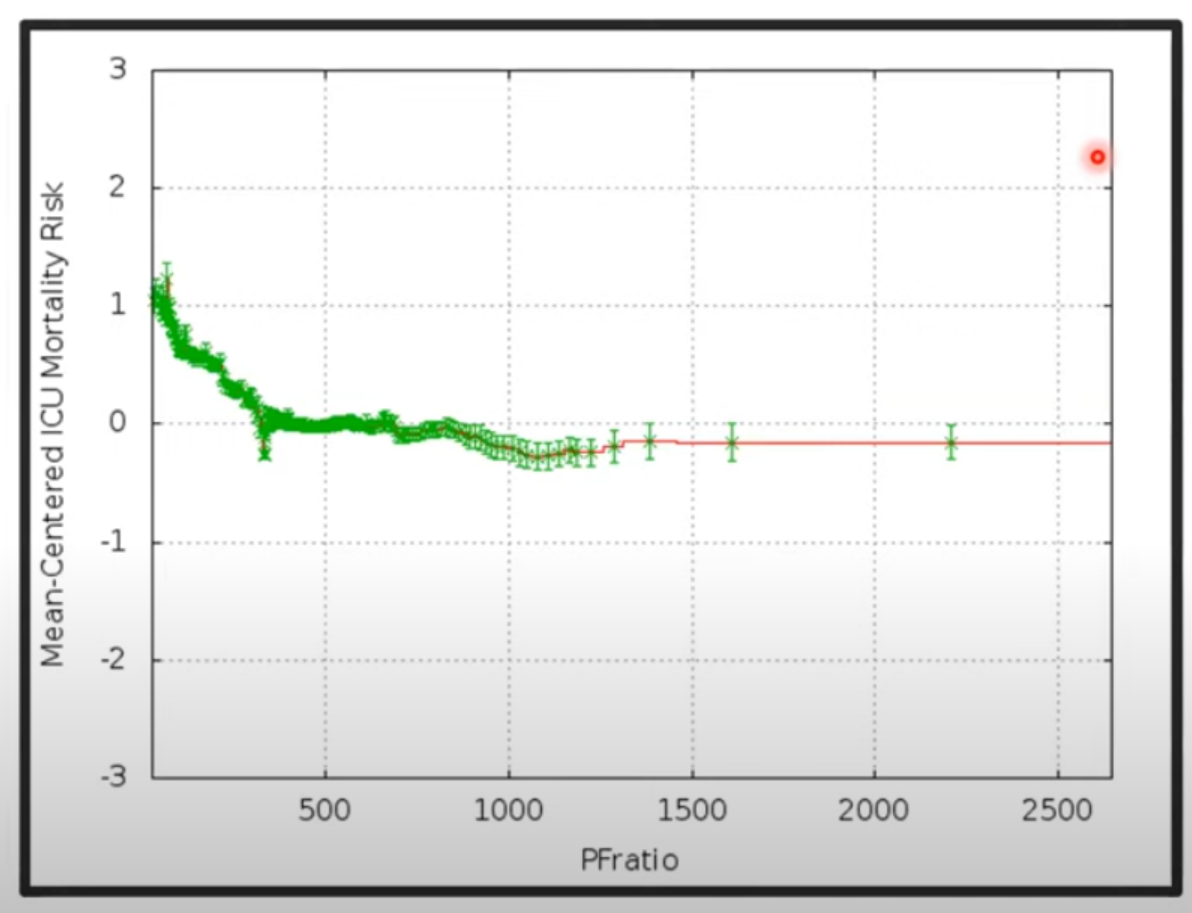
\includegraphics[width=0.5\linewidth]{slides/07_imputation/figure_man/Screenshot from 2025-06-03 22-38-17.png}
    \caption{Figure from Rich Caruana's talk at the AutoML conference 2024, example starting at 43'31 \href{https://www.youtube.com/watch?v=5mH7Fyy5wQY}{\beamergotobutton{REF}}}
\end{figure}
\vfill
\end{frame}

\begin{frame}{A tale of failed imputation 2}
\vfill
\begin{figure}
    \centering
    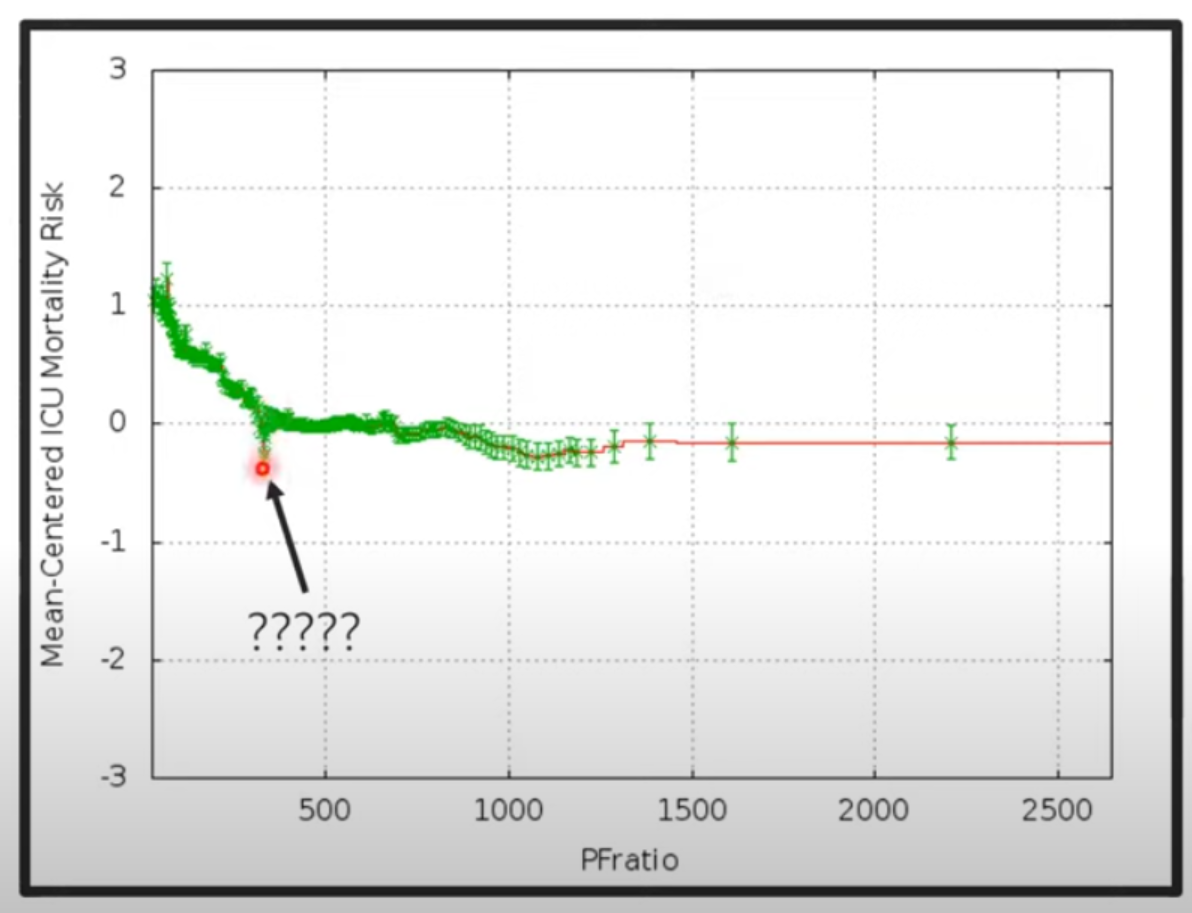
\includegraphics[width=0.5\linewidth]{slides/07_imputation/figure_man/Screenshot from 2025-06-03 22-38-27.png}
    \caption{Figure from Rich Caruana's talk at the AutoML conference 2024, example starting at 43'31 \href{https://www.youtube.com/watch?v=5mH7Fyy5wQY}{\beamergotobutton{REF}}}
\end{figure}
\vfill    
\end{frame}

\begin{frame}{A tale of failed imputation 3}
\vfill
\begin{figure}
    \centering
    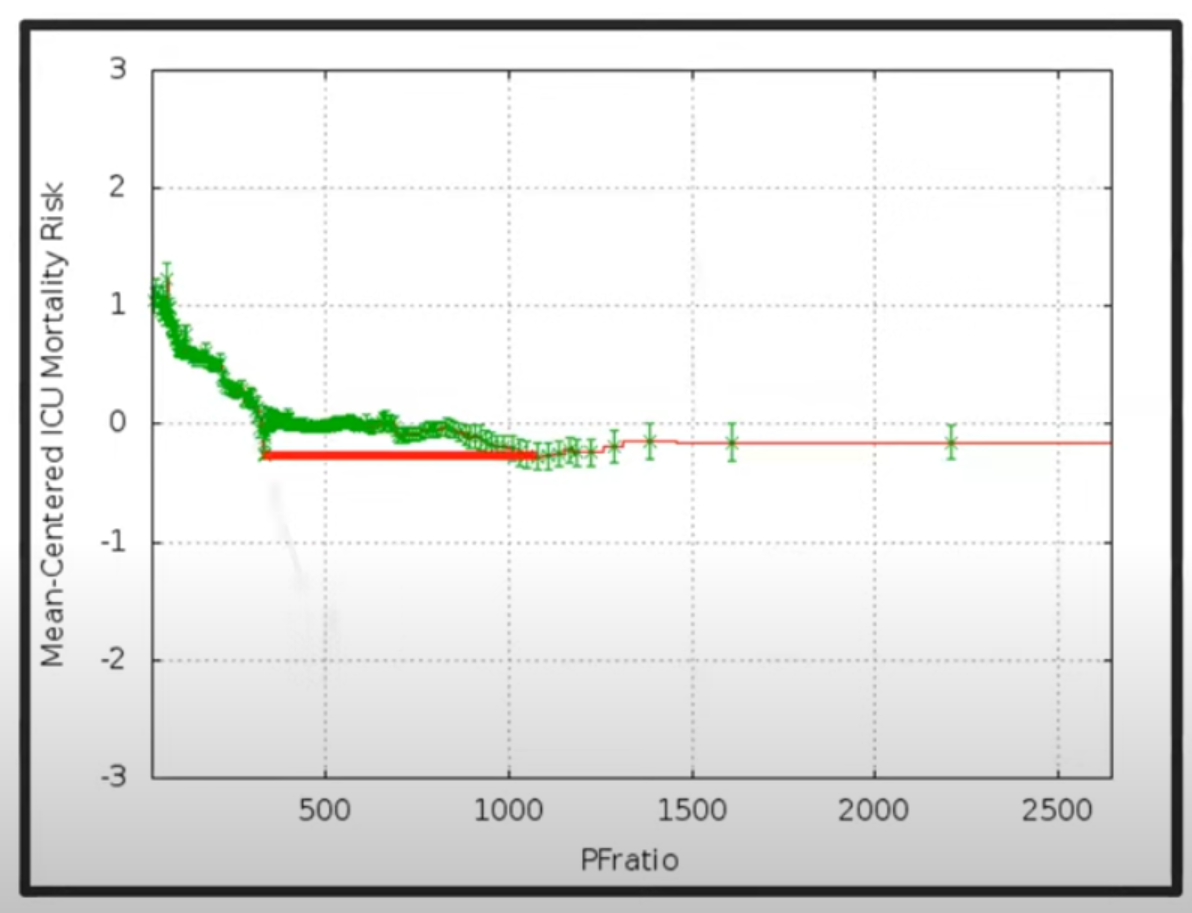
\includegraphics[width=0.5\linewidth]{slides/07_imputation/figure_man/Screenshot from 2025-06-03 22-38-34.png}
    \caption{Figure from Rich Caruana's talk at the AutoML conference 2024, example starting at 43'31 \href{https://www.youtube.com/watch?v=5mH7Fyy5wQY}{\beamergotobutton{REF}}}
\end{figure}
\vfill
\end{frame}

\begin{frame}{A tale of failed imputation 4}
\vfill
\begin{figure}
    \centering
    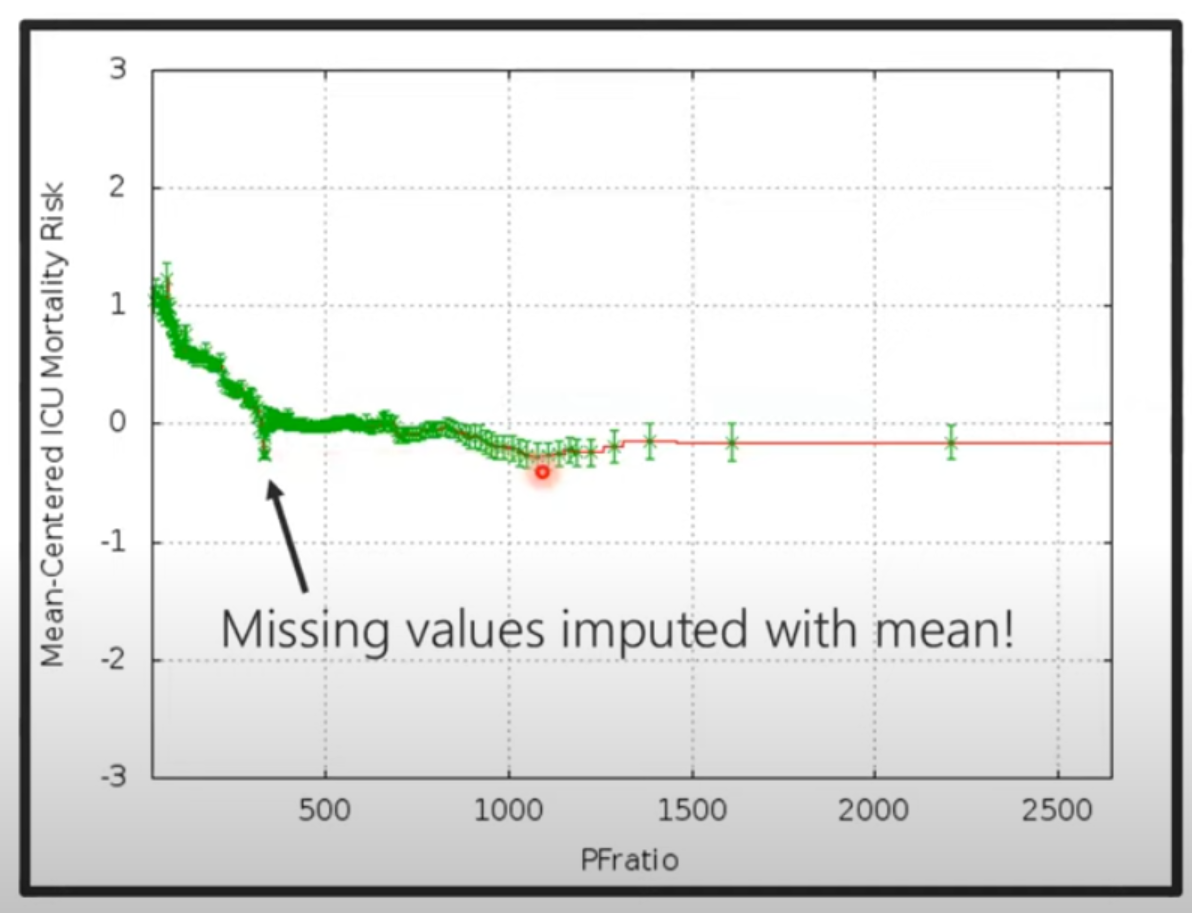
\includegraphics[width=0.5\linewidth]{slides/07_imputation/figure_man/Screenshot from 2025-06-03 22-38-41.png}
    \caption{Figure from Rich Caruana's talk at the AutoML conference 2024, example starting at 43'31 \href{https://www.youtube.com/watch?v=5mH7Fyy5wQY}{\beamergotobutton{REF}}}
\end{figure}
\vfill
\end{frame}

\begin{frame}{A tale of failed imputation 5}
\vfill
\begin{figure}
    \centering
    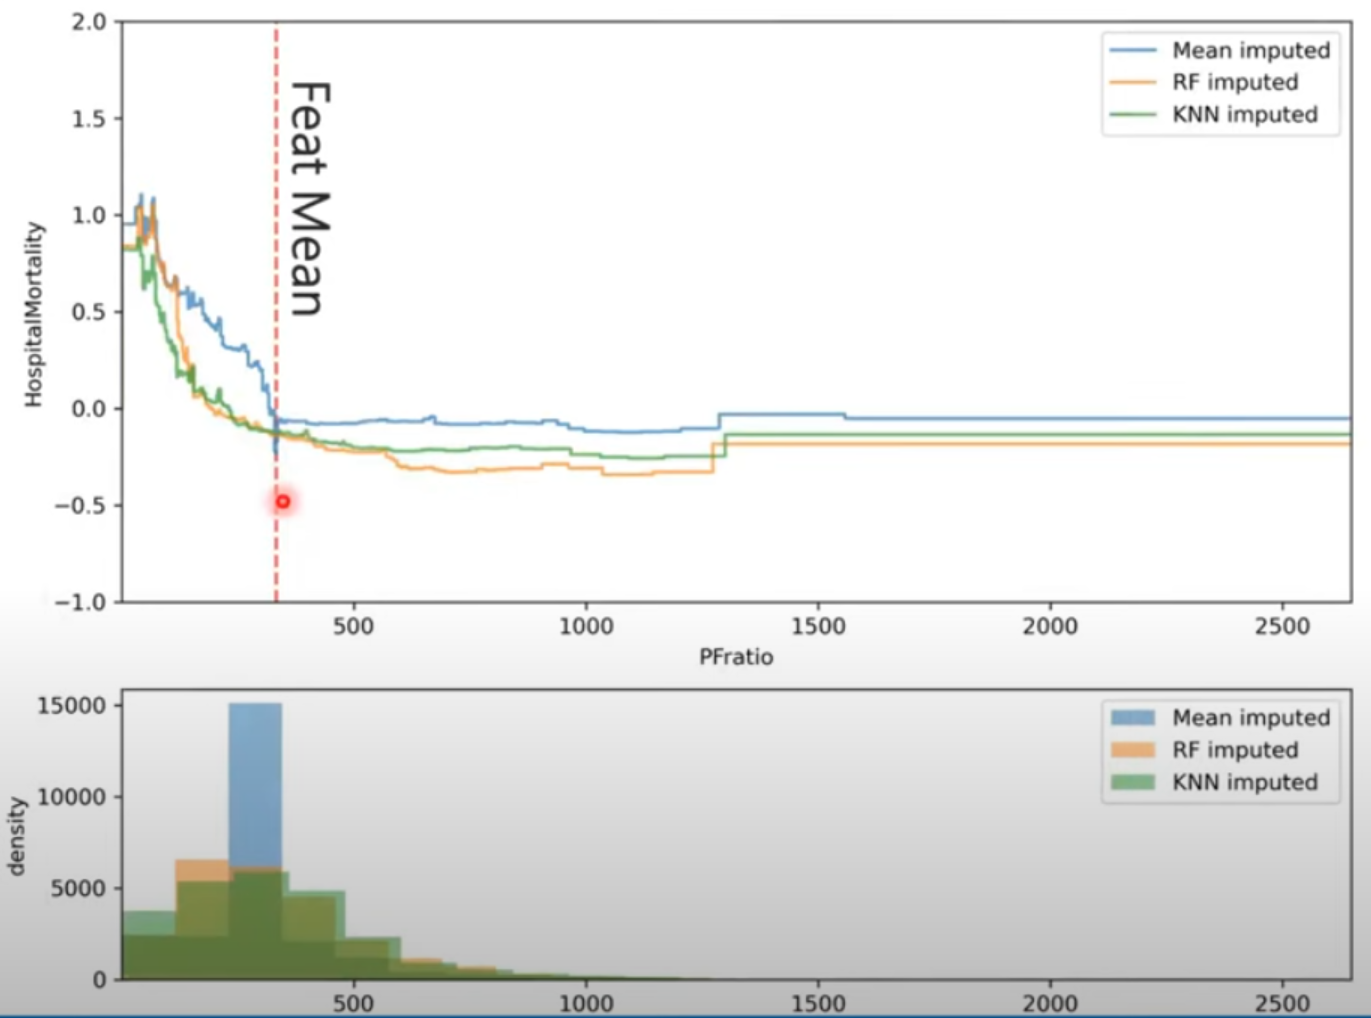
\includegraphics[width=0.5\linewidth]{slides/07_imputation/figure_man/Screenshot from 2025-06-03 22-39-01.png}
    \caption{Figure from Rich Caruana's talk at the AutoML conference 2024, example starting at 43'31 \href{https://www.youtube.com/watch?v=5mH7Fyy5wQY}{\beamergotobutton{REF}}}
\end{figure}
\vfill
\end{frame}

\begin{frame}{Tests for missingness mechanisms}
\vfill
MAR vs MCAR
\begin{itemize}
    \vfill
    \item Little's test
    \item Logistic regression for missingness
    \begin{enumerate}
        \item For each column, create a new classification task: predict if the value is missing or not
        \item Use the remaining columns as features
        \item Fit logistic regression
        \item Examine coefficients and p-values
    \end{enumerate}
    \vfill
\end{itemize}
MNAR: no test available
\vfill
\end{frame}

\begin{frame}{Censored data: special missingness mechanisms}
    \small
    \begin{itemize}
        \item Left censoring – a data point is below a certain value but it is unknown by how much.
        \item Interval censoring – a data point is somewhere on an interval between two values.
        \item Right censoring – a data point is above a certain value but it is unknown by how much.
        \item Type I censoring occurs if an experiment has a set number of subjects or items and stops the experiment at a predetermined time, at which point any subjects remaining are right-censored.
        \item Type II censoring occurs if an experiment has a set number of subjects or items and stops the experiment when a predetermined number are observed to have failed; the remaining subjects are then right-censored.
        \item Random (or non-informative) censoring is when each subject has a censoring time that is statistically independent of their failure time. The observed value is the minimum of the censoring and failure times; subjects whose failure time is greater than their censoring time are right-censored.
    \end{itemize}
\end{frame}

\begin{frame}{Takeaways of a recent benchmark}

Imputation for prediction: beware of diminishing return. Le Morvan and Varoquaux, ICLR 2025 \href{https://arxiv.org/pdf/2407.19804}{\beamergotobutton{REF}}

\begin{itemize}
    \item Better imputation performance does not result in better prediction performance for MNAR (w/o missingness indicator)
    \item Better imputation might be irrelevant b/c information is available in other features, unimportant, even with imputation it might be hard to learn a good downstream model
    \item More expressive models have less (relative) benefit from imputation
    \item Best on average: missForest + XGBoost + masking
    \item Open Questions:
    \begin{itemize}
        \item performance of random draws
        \item performance of multiple imputation
        \item impact of performance on explainability and calibration
        \item performance of models that can learn directly with missing value (advanced transformer architectures)
    \end{itemize}
\end{itemize}
    
\end{frame}

\begin{frame}{Takeaways}
    \vfill
    \begin{itemize}
        \item There exist different reasons for missing data
        \item There exist different missingness mechanisms
        \item Different downstream tasks ask for different imputation strategies
        \item Different data modalities ask for different imputation strategies
        \item Understanding the data generating process helps deciding on the imputation strategy
        \item Common imputation strategies:
        \begin{itemize}
            \item Constant value: mean, median
            \item Imputation by sampling
            \item Missingness indicator
            \item Model-based
        \end{itemize}
        $\rightarrow$ imputation selection is a CASH problem
    \end{itemize}
    \vfill
\end{frame}

\endlecture
\end{document}
